\documentclass[11pt, twocolumn, a4paper]{article}
\usepackage[a4paper, left = 2cm, right = 2cm, top = 2cm, bottom = 2cm]{geometry}
\usepackage[style = numeric, sorting = none, urldate = long]{biblatex}
\usepackage{listings}
\usepackage{subfig}
\usepackage{pgfplots}
\usepackage[T1]{fontenc}


% \graphicspath{{./images/}}
\addbibresource{refs.bib}

\author{
    George Herbert\\
    \texttt{cj19328@bristol.ac.uk}
}

\title{Optimising and Parallelising d2q9-bgk.c}
\begin{document}

\maketitle

\begin{abstract}
    \texttt{d2q9-bgk.c} implements the Lattice Boltzmann methods (LBM) to simulate a fluid density on a lattice.
    This report outlines the techniques I utilised to optimise and parallelise \texttt{d2q9-bgk.c}, as well as a detailed analysis of those techniques.
    To do so, this report is split into several sections corresponding to different iterations of my code.
\end{abstract}

\section{Original Code}

I compiled the original \texttt{d2q9-bgk.c} using the GNU Compiler Collection (GCC) with the following command:
\begin{lstlisting}[language=bash, breaklines=true, breakatwhitespace=true]
gcc -std=c99 -Wall -O3 d2q9-bgk.c -lm -o d2q9-bgk.
\end{lstlisting}

\begin{table}[htbp]
    \begin{center}
    \caption{Execution times of the original code}\label{tab:original}
    \begin{tabular}{l | l} 
        \hline\hline
        Test Case Size&Time (s)\\
        \hline
        $128 \times 128$&\texttt{ 29.16}\\
        $128 \times 256$&\texttt{ 58.71}\\
        $256 \times 256$&\texttt{233.32}\\
        $1024 \times 1024$&\texttt{980.89}\\
        \hline
      \end{tabular}
    \end{center}
\end{table} 

Table \ref{tab:original} contains the total time to initialise, compute and collate each of the test cases when running the ELF file produced.
It was important to measure the original code, so that I could quantify the performance improvements of my latter implementations.
I measured each of the total times by taking an average of 10 runs on BlueCrystal Phase 4's (BC4's) compute nodes.
Each of BC4's compute nodes was a Lenovo nx360 M5, which contained two 14-core 2.4 GHz Intel E5-2680 v4 (Broadwell) CPUs and 128 GiB of RAM \cite{bcp4}.
I took an average of multiple runs because of the variation between runs, which existed due to the inconsistent performance of compute nodes.
% Not all compute nodes offer the same performance all of the time, due to differing placement in the data centre, amongst other reasons.

\section{Serial Optimisations}

I initially implemented a collection of serial optimisations to improve the performance of \texttt{d2q9-bgk.c}.

\subsection{Compiler}

The first improvement I implemented was compiling with the Intel C Compiler as opposed to GCC, since it produced better optimised code for Intel processors.
Furthermore, I compiled my code with the \texttt{Ofast} option, which set aggressive options to improve the speed of my program, including \texttt{O3} optimisations and aggressive floating point optimisations \cite{icc}.

\begin{table}[htbp]
  \begin{center}
  \caption{Execution times after compiler changes, and speedup over the original code}\label{tab:compiler_changes}
  \begin{tabular}{l | l l} 
      \hline\hline
      Grid Size&Time (s)&Speedup\\
      \hline
      $128 \times 128$&\texttt{ 22.25}&\texttt{1.31}\\
      $128 \times 256$&\texttt{ 44.42}&\texttt{1.32}\\
      $256 \times 256$&\texttt{176.69}&\texttt{1.33}\\
      $1024 \times 1024$&\texttt{795.41}&\texttt{1.23}\\
      \hline
    \end{tabular}
  \end{center}
\end{table}

These changes to the compilation process provided a reasonable performance boost, as shown in Table \ref{tab:compiler_changes}.

\subsection{Loop Fusion and Pointer Swap}

For all the test cases provided, the implementation of LBM in \texttt{d2q9-bgk} was a memory bound problem.
As a result of this, there was a significant opportunity to optimise \texttt{d2q9-bgk.c} by decreasing the number of memory accesses.
One method I utilised to accomplish this was loop fusion.
In the original code, the entire grid was iterated over in four sequential procedures within each timestep: \texttt{propagate}, \texttt{rebound}, \texttt{collision} and \texttt{av\_velocity}.
By absorbing these four procedures into the \texttt{timestep} procedure and fusing the four loops, I was able to drastically decrease the number of memory accesses, thereby improving the performance of my program.

Implementing loop fusion offered another significant opportunity to eliminate redundant memory accesses.
The original code had a significant quantity of value copying between the \texttt{cells} and \texttt{tmp\_cells} arrays.
I was able to eliminate this by writing all new values of cells to a \texttt{cells\_new} array, and simply swapping the pointers of \texttt{cells\_new} and \texttt{cells} at the end of each timestep.
I eliminated the \texttt{tmp\_cells} array entirely.

\begin{table}[htbp]
  \begin{center}
  \caption{Execution times after loop fusion and pointer swap, and speedup over the original code}\label{tab:loop_fusion_pointer_swap}
  \begin{tabular}{l | l l} 
      \hline\hline
      Test Case Size&Time (s)&Speedup\\
      \hline
      $128 \times 128$&\texttt{ 19.42}&\texttt{1.50}\\
      $128 \times 256$&\texttt{ 39.21}&\texttt{1.50}\\
      $256 \times 256$&\texttt{155.64}&\texttt{1.50}\\
      $1024 \times 1024$&\texttt{635.61}&\texttt{1.54}\\
      \hline
    \end{tabular}
  \end{center}
\end{table}

Decreasing the number of memory accesses provided further performance improvements, as shown in Table \ref{tab:loop_fusion_pointer_swap}.

\subsection{Arithmetic Improvements}

Despite the compiler being able to partially optimise the arithmetic within each timestep without making any changes to the code, there were still some manual improvements that I made to improve the performance of the program.
Division is a very slow arithmetic operation relative to multiplication.
Therefore, to eliminate a large number of unnecessary division operations I precalculated several values including:
\[
    \frac{1}{c^2} = 3\qquad
    \frac{1}{2c^2} = 1.5\qquad
    \frac{1}{2c^4} = 4.5
\]
where $c$ is the speed of sound.
Additionally, I noticed that the number of cells in the grid that were not obstacles \texttt{tot\_u} was recalculated and then divided by each timestep.
I eliminated this inefficiency by counting number of cells that were not obstacles only once (during the initialisation phase).
I then saved the reciprocol of this value as a parameter \texttt{num\_non\_obstacles\_r}, which I used once per timestep in a multiplicative operation to compute the average velocity.

\begin{table}[htbp]
  \begin{center}
  \caption{Execution times after arithmetic improvements, and speedup over the original code}\label{tab:arithmetic_improvements}
  \begin{tabular}{l | l l} 
      \hline\hline
      Test Case Size&Time (s)&Speedup\\
      \hline
      $128 \times 128$&\texttt{ 19.10}&\texttt{1.53}\\
      $128 \times 256$&\texttt{ 38.49}&\texttt{1.53}\\
      $256 \times 256$&\texttt{153.39}&\texttt{1.52}\\
      $1024 \times 1024$&\texttt{621.52}&\texttt{1.58}\\
      \hline
    \end{tabular}
  \end{center}
\end{table}

These arithmetic improvements provided only a small boost to performance compared to the prior implementation, as shown in Table \ref{tab:arithmetic_improvements}.
This was to be expected since the Intel C Compiler had already optimised a large amount of the arithmetic.

\subsection{Vectorization}

Vectorization is the process of converting a scalar implementation to a vector implementation, which enables the compiler to make use of additional registers to perform multiple operations in a single instruction \cite{vectorization}.
I utilised several techniques to enforce single-instruction-multiple-data (SIMD) vectorization of the inner loop within each timestep.

Firstly, I converted the \texttt{t\_speed} structure holding cell speeds from an array of structures (AoS) to a structure of arrays (SoA).
Previously, the grid was represented with an array of \texttt{t\_speed} structures, whereby each structure contained nine vectors (represented by an array of nine floats).
I altered this such that the grid was represented by one \texttt{t\_speed} structure containing nine pointers, each to an individual array of floats.
Each array of floats contained the values of one vector for each cell within the grid.
The SoA format greatly suited vectorization of the inner loop, since it kept memory accesses contiguous when vectorization was performed over structure instances \cite{soa}.

Having altered the data layout to suit vectorization, I utilised several other techniques to enforce vectorization.
Within my code, I implemented the \texttt{\#pragma omp simd} pragma to vectorise the inner loop within each timestep.
This pragma indicated to the compiler that SIMD instructions could be used to execute iterations of the loop concurrently.
The \texttt{qopenmp-simd} option is enabled by default at optimisation levels of \texttt{O2} or higher to enable OpenMP SIMD compilation \cite{icc}.
Furthermore, I utilised the \texttt{reduction(+:tot\_u)} clause to ensure the \texttt{tot\_u} variable contained the correct value at the loop's termination.

I used the \texttt{restrict} keyword in \texttt{timestep}'s parameters for the \texttt{cells}, \texttt{cells\_new} and \texttt{obstacles} variables.
This asserted that the memory referenced by pointers to these variables was not aliased.
I compiled my program with the \texttt{restrict} option to enable pointer disambiguation for these variables.
Overall, this provided a performanced advantage as it prevented the compiler from performing a runtime test for aliasing.

Processors are designed to efficiently move data located on specific byte boundaries, and the compiler is able to perform optimisations when data access is known to be aligned by 64 bytes \cite{alignment}.
To align the \texttt{cells}, \texttt{cells\_new} and \texttt{obstacles} variables, I replaced calls to the \texttt{malloc} and \texttt{free} procedures with the alignment specific replacements: \texttt{\_mm\_malloc} and \texttt{\_mm\_free}, respectively.
I used the \texttt{\_\_assume\_\_aligned} procedure and  the statement \texttt{\_\_assume(params.nx \% 16 == 0)} to inform the compiler that the dynamically allocated variables were aligned.
Doing so prevented the compiler from generating conservative code, which would have been detrimental to performance.

Once I had utilised these techniques to enforce efficient vectorization of the inner loop, I compiled \texttt{d2q9-bgk.c} with the \texttt{xAVX2} option to direct the compiler to optimise for Intel processors that support Advanced Vector Extensions 2 (AVX2), as BC4's compute nodes do \cite{lenovo}.

\begin{table}[htbp]
  \begin{center}
  \caption{Execution times after vectorization, and speedup over the original code}\label{tab:vectorized}
  \begin{tabular}{l | l l} 
      \hline\hline
      Test Case Size&Time (s)&Speedup\\
      \hline
      $128 \times 128$&\texttt{  \,\,\,5.77}&\texttt{5.05}\\
      $128 \times 256$&\texttt{ 11.57}&\texttt{5.07}\\
      $256 \times 256$&\texttt{ 41.55}&\texttt{5.62}\\
      $1024 \times 1024$&\texttt{215.52}&\texttt{4.55}\\
      \hline
    \end{tabular}
  \end{center}
\end{table}

Vectorization provided the largest performance improvement of any optimisation that I had implemented to this point, as shown in Table \ref{tab:vectorized}.
This made sense in theory, since AVX2 could perform simultaneous operations on up to eight single precision floating point numbers, thereby vastly decreasing the quantity of time spent in the vectorized inner loop.

\section{Parallelism}

Overall, my serial optimisations (including vectorization) achieved approximately a five times speedup over the original implementation.
However, there was a large potential for performance improvements by parallelising \texttt{d2q9-bgk.c}. 

\subsection{OpenMP}

OpenMP implements parallelism by launching a set of threads that execute portions of code concurrently \cite{openmp_cornell}.
I utilised OpenMP's \texttt{\#pragma omp parallel for} pragma to direct the compiler to parallelise the outer loop in the \texttt{timestep} procedure.
Furthermore, I compiled my code with the \texttt{qopenmp} option, which enabled the paralellizer to generate multi-threaded code based on OpenMP directives, as that which I defined.
Since the \texttt{tot\_u} variable needed to contain the total velocities of each cell, I used the clause \texttt{reduction(+:tot\_u)} to prevent race conditions.
This informed the compiler to create a copy of the \texttt{tot\_u} variable for each thread (initialised to zero), and to sum the local results when the outer loop terminates.

\begin{table}[htbp]
  \begin{center}
  \caption{Execution times after parallelising (run with 28 threads), and speedup over both the original and vectorized code}\label{tab:parallelised}
  \begin{tabular}{l | l  l  l} 
      \hline\hline
      &&\multicolumn{2}{c}{Speedup}\\
      \cline{3-4}
      Grid Size&Time (s)&Original&Vectorized\\
      \hline
      $128 \times 128$&\texttt{ 1.30}&\texttt{22.43}&\texttt{ 4.44}\\
      $128 \times 256$&\texttt{ 1.48}&\texttt{39.67}&\texttt{ 7.82}\\
      $256 \times 256$&\texttt{ 3.61}&\texttt{64.63}&\texttt{11.51}\\
      $1024 \times 1024$&\texttt{16.93}&\texttt{57.94}&\texttt{12.73}\\
      \hline
    \end{tabular}
  \end{center}
\end{table}

Table \ref{tab:parallelised} displays the execution times for my parallel implementation (run with 28 threads), and speedup over both the original and vectorized code.

\subsection{Non-Uniform Memory Access (NUMA)}

NUMA is a computer memory design in which memory access time depends on the memory location relative to the processor \cite{numa}.
Memory is allocated to the closest NUMA region to the thread that first touches the data \cite{numa_bristol}.
Since BC4's compute nodes contain two sockets, the memory access time for a given thread primarily depends on whether the memory is connected to the socket the thread resides in or not.
I parallelised the initialisation loops for \texttt{cells} and \texttt{obstacles} to ensure that each thread touched the same data in both the \texttt{initialise} and \texttt{compute} procedures.
Furthermore, I set the environment variables \texttt{OMP\_PROC\_BIND=true} and \texttt{OMP\_PLACES=cores} to prevent threads from moving cores.

\begin{table}[htbp]
  \begin{center}
  \caption{Execution times after writing NUMA-aware implementation (run with 28 threads), and speedup over both the original and vectorized code}\label{tab:numa}
  \begin{tabular}{l | l  l  l} 
      \hline\hline
      &&\multicolumn{2}{c}{Speedup}\\
      \cline{3-4}
      Grid Size&Time (s)&Original&Vectorized\\
      \hline
      $128 \times 128$&\texttt{ 0.71}&\texttt{41.07}&\texttt{ 8.13}\\
      $128 \times 256$&\texttt{ 0.82}&\texttt{71.60}&\texttt{14.11}\\
      $256 \times 256$&\texttt{ 2.64}&\texttt{88.38}&\texttt{15.73}\\
      $1024 \times 1024$&\texttt{13.47}&\texttt{72.82}&\texttt{16.00}\\
      \hline
    \end{tabular}
  \end{center}
\end{table}

Table \ref{tab:numa} contains the updated execution times for my final NUMA-aware implementation.
As anticipated, parallelising the initialisation loops and preventing threads from moving cores provided a modest boost to performance.

\subsection{Scaling}

I ran my final, NUMA-aware implementation from one to 28 threads to gain an insight into how my implementation scaled.

\begin{figure}[htpb]
  \centering
  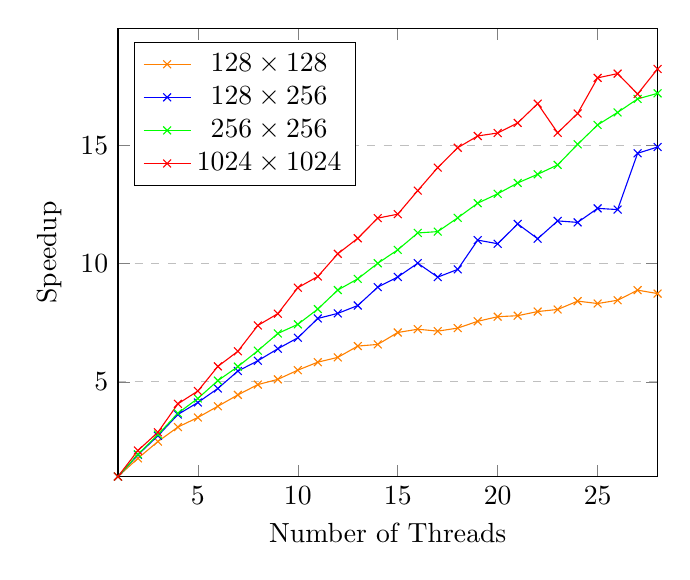
\begin{tikzpicture}
    \begin{axis}[
      xlabel={Number of Threads},
      ylabel={Speedup},
      xmin = 1, xmax = 28,
      ymin = 1,
      % xtick={0, 5, 10, 15, 20, 25},
      % ytick={0,20,40,60,80,100,120},
      legend pos=north west,
      ymajorgrids=true,
      grid style=dashed,
    ]
    \addlegendentry{$128\times128$}
    \addplot[color = orange, mark = x]coordinates{
      (1, 1)
      (2, 1.770147781)
      (3, 2.479203736)
      (4, 3.090127044)
      (5, 3.495898299)
      (6, 3.969781807)
      (7, 4.449517419)
      (8, 4.885230537)
      (9, 5.105636521)
      (10, 5.495622472)
      (11, 5.832498588)
      (12, 6.033959916)
      (13, 6.511971973)
      (14, 6.581786272)
      (15, 7.08579377)
      (16, 7.224322206)
      (17, 7.143221767)
      (18, 7.27187543)
      (19, 7.559142588)
      (20, 7.752570216)
      (21, 7.795101063)
      (22, 7.970592183)
      (23, 8.058757757)
      (24, 8.411400223)
      (25, 8.309209659)
      (26, 8.448042356)
      (27, 8.873950316)
      (28, 8.729508452)
    };
    \addlegendentry{$128\times256$}
    \addplot[color = blue, mark = x]coordinates{
      (1, 1)
      (2, 1.918812078)
      (3, 2.722691991)
      (4, 3.620768356)
      (5, 4.129091999)
      (6, 4.720896994)
      (7, 5.457129627)
      (8, 5.890235496)
      (9, 6.398711601)
      (10,6.861778085)
      (11,7.679664463)
      (12,7.892142111)
      (13,8.225546911)
      (14,9.002082643)
      (15,9.431524198)
      (16,10.01307455)
      (17,9.424918639)
      (18,9.751774957)
      (19,10.9890841)
      (20,10.83510235)
      (21,11.67306753)
      (22,11.04704628)
      (23,11.80091066)
      (24,11.73689961)
      (25,12.3300502)
      (26,12.27839835)
      (27,14.65659506)
      (28,14.92261783)
    };
    \addlegendentry{$256\times256$}
    \addplot[color = green, mark = x]coordinates{
      (1, 1)
      (2, 1.938375582)
      (3, 2.771151595)
      (4, 3.675722466)
      (5, 4.299722521)
      (6, 5.052146164)
      (7, 5.643422171)
      (8, 6.316100162)
      (9, 7.04401679)
      (10, 7.429468926)
      (11, 8.075812314)
      (12, 8.879274603)
      (13, 9.352559102)
      (14, 10.00947825)
      (15, 10.57828753)
      (16, 11.29099838)
      (17, 11.34786525)
      (18, 11.9302309)
      (19, 12.54826914)
      (20, 12.94577227)
      (21, 13.4034522)
      (22, 13.76922924)
      (23, 14.16603038)
      (24, 15.03635571)
      (25, 15.85516854)
      (26, 16.38362619)
      (27, 16.95314186)
      (28, 17.18947447)

    };
    \addlegendentry{$1024\times1024$}
    \addplot[color = red, mark = x]coordinates{
      (1, 1)
      (2, 2.100760194)
      (3, 2.870122668)
      (4, 4.071422641)
      (5, 4.614599066)
      (6, 5.652837154)
      (7, 6.291146923)
      (8, 7.383068123)
      (9, 7.881869892)
      (10, 8.977180241)
      (11, 9.452161408)
      (12, 10.41116263)
      (13, 11.06645567)
      (14, 11.91753689)
      (15, 12.0840354)
      (16, 13.08055546)
      (17, 14.05218119)
      (18, 14.89108656)
      (19, 15.38824382)
      (20, 15.51458921)
      (21, 15.93993521)
      (22, 16.75254912)
      (23, 15.52257546)
      (24, 16.33948228)
      (25, 17.84378604)
      (26, 18.02294074)
      (27, 17.16198512)
      (28, 18.21858148)
    };
    \end{axis}
  \end{tikzpicture}
  \caption{Speedup curves for my NUMA-aware implementation}\label{fig:scaling}
\end{figure}

I plotted the amount of speedup over the single thread implementation that different quantities of threads provided.
The resulting speedup curves for each test case are displayed in Figure \ref{fig:scaling}.
For each grid size, my implementation initially scales well, but the performance aquired from each subsequent core begins to decline.
This is known as a sublinear plateau.

\clearpage

\onecolumn{
  \printbibliography
}

\end{document}